\documentclass{standalone}

\usepackage{tikz}
    % \usetikzlibrary{calc}
    
\begin{document}
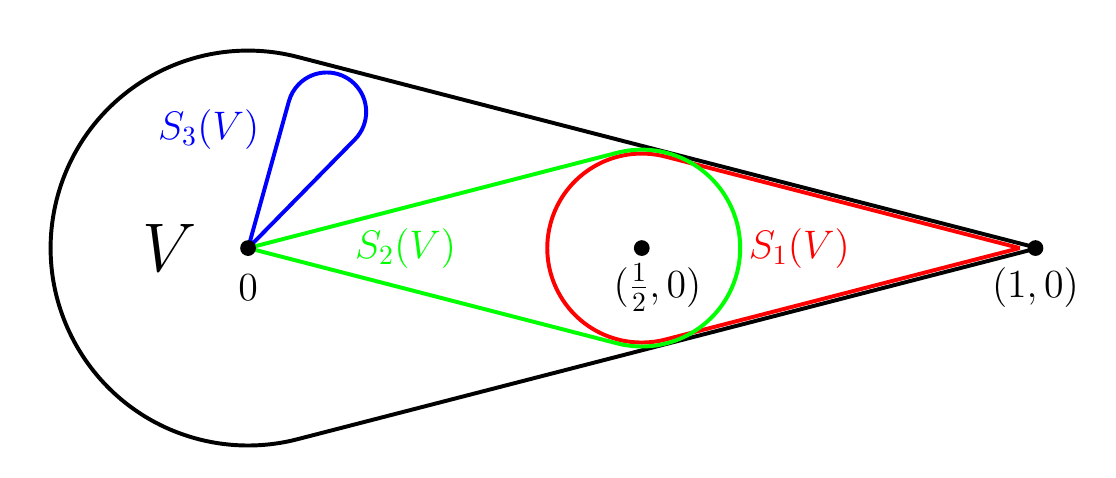
\begin{tikzpicture}
    % \draw[help lines] (-3,-3) grid (10,3);
    \foreach \o/\k/\t/\c in
        {(0,0)/10.03/0/black, (5,0)/4.8/0/red, (5,0)/5/180/green, (1,1.73)/2/240/blue} 
        {\draw[line width=0.5mm, \c] 
            \o+(75.52+\t:\k/4) -- +(\t:\k)
            \o+(284.47+\t:\k/4) -- +(\t:\k)
            \o+(75.52+\t:\k/4) arc (75.52+\t:284.47+\t:\k/4);}
    \node[shift={(-1,0)}] {\Huge$V$};
    \node[shift={(0,-.5)}] {\Large$0$};
    \node[shift={(5.2,-.5)}] {\Large$(\frac{1}2,0)$};
    \node[shift={(10,-.5)}] {\Large$(1,0)$};
    \node[shift={(-0.5,1.5)},blue] {\Large$S_3(V)$};
    \node[shift={(2,0)},green] {\Large$S_2(V)$};
    \node[shift={(7,0)},red] {\Large$S_1(V)$};
    \fill[black] 
        (0,0)circle(0.1)
        (5,0)circle(0.1)
        (10,0)circle(0.1);
\end{tikzpicture}
\end{document}